% !TEX root=../presentation_1.tex
\section{Introduction}

\subsection{Minimum-Weight Spanning Tree (MST)}

\begin{frame}
\frametitle{Minimum-Weight Spanning Tree (MST)}

\begin{itemize}
  \item A \textbf{weighted} graph $G = (V,E,W)$. $V$ is a set of vertices and $E$ is a set of edges, and each edge has an associated weight.
  \item A \textbf{spanning tree} is a tree that covers all vertices.
  \item A spanning tree is \textbf{minimum} if the sum of all weights in the tree is the minimum among all spanning trees.
\end{itemize}
\begin{figure}
    \centering
    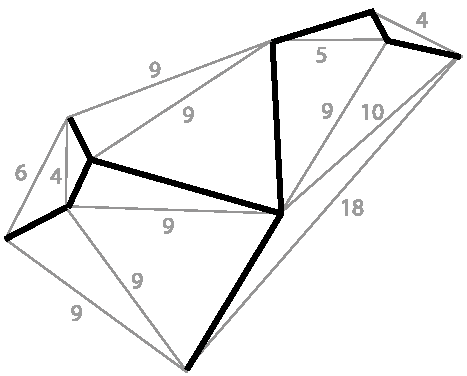
\includegraphics[width=0.4\textwidth]{figures/mst.pdf}
    \caption{An example of MST}
\end{figure}
\end{frame}

\subsection{Practical Applications}

\begin{frame}
\frametitle{Practical Applications}
\begin{itemize}
  \item Building highways.
  \item Building network links.
  \item Broadcasting.
  \item Circuit design.
  \item Clustering, image segmentation.
\end{itemize}
\begin{figure}
    \centering
    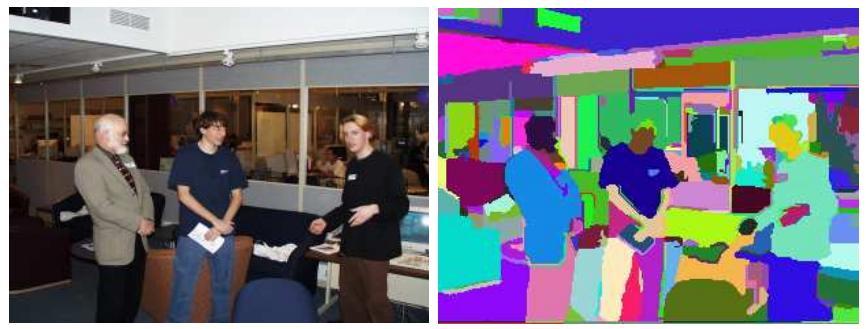
\includegraphics[width=0.6\textwidth]{figures/segmentation.png}
    \caption{An MST-based Image Segmentation Method [FH04]}
\end{figure}
\end{frame}

\subsection{Greedy Sequential Algorithms}

\begin{frame}
\frametitle{Greedy Sequential Algorithms}

\begin{itemize}
\item \textcolor{red}{\textbf{Red}} rule. Let $C$ be a cycle with no red arcs. Select an uncolored arc of $C$ of max weight and color it red. 
\item \textcolor{blue}{\textbf{Blue}} rule. Let $D$ be a cut with no blue arcs. Select an uncolored arc in $D$ of min weight and color it blue.
\end{itemize}
\begin{itemize}
  \item Boruvka's algorithm
    \begin{itemize}
      \item The first MST algorithm developed in the 20s.
      \item Iteratively merging MST forest.
    \end{itemize}
  \item Kruskal's algorithm
    \begin{itemize} 
      \item Iteratively adding minimum weighted edge without forming a cycle.
    \end{itemize}
  \item Prim's algorithm
    \begin{itemize} 
      \item Iteratively expanding the vertices by selecting the minimum weighted outgoing edge.
    \end{itemize}
\end{itemize}
\end{frame}


\begin{frame}
\animategraphics{12}{figures/KruskalDemo-}{0}{9}
\end{frame}